\section{问题二：库存约束下的离线模型}\label{sec:q2}

\subsection{含库存约束的流体线性规划}
题目中的 hindsight 模型以 $x_{ij}\in\{0,1\}$ 表示是否向类型 $i$ 推荐商品 $j$，目标函数为 $\sum_i\sum_jN_ir_jp_{ij}x_{ij}$，每类顾客至多获得 $K$ 件推荐。引入库存后需要做两处修改。其一，整个销售期内商品 $j$ 的期望销量 $\sum_iN_ip_{ij}x_{ij}$ 不超过初始库存 $C_j$。其二，把 $x_{ij}$ 放松为 $[0,1]$ 内的比例：同一类型的不同顾客可以看到不同的推荐集合，$x_{ij}$ 表示类型 $i$ 的顾客中看到商品 $j$ 的比例。令 $y_{ij}=N_ix_{ij}$ 表示向类型 $i$ 推荐商品 $j$ 的期望次数，得到离线流体线性规划
\begin{equation}
\begin{aligned}
F(N,C)=\max_{y}\quad &\sum_{i=1}^{m}\sum_{j=1}^{n}r_jp_{ij}\,y_{ij}\\
\mathrm{s.t.}\quad &\sum_{i=1}^{m}p_{ij}\,y_{ij}\le C_j, &&j=1,\ldots,n, &&(\beta_j)\\
&\sum_{j=1}^{n}y_{ij}\le K N_i, &&i=1,\ldots,m, &&(\mu_i)\\
&0\le y_{ij}\le N_i, &&i=1,\ldots,m,\ j=1,\ldots,n.
\end{aligned}
\label{eq:lp}
\end{equation}
第一组约束要求商品 $j$ 的期望销量不超过库存；第二组约束表示类型 $i$ 的 $N_i$ 位顾客最多提供 $KN_i$ 个推荐位；变量上界表示每位顾客至多看到同一商品一次。模型含 $mn$ 个连续变量和 $m+n$ 条约束，课程实例为 9 个变量、6 条约束。到达序列只通过人数向量 $N$ 进入模型，五份数据的人数相同，离线最优值都等于 $F\bigl((50,30,20),C\bigr)$。本文取 $\mathrm{OPT}_{\mathrm{hind}}=F(N,C)$。

\begin{proposition}\label{prop:upper}
对任意到达序列 $i_{1:T}$ 与任意满足约束\eqref{eq:feasible}的在线策略 $\pi$，
\begin{equation}
\E\bigl[R_T(\pi)\mid i_{1:T}\bigr]\le F(N,C).
\label{eq:upper}
\end{equation}
\end{proposition}
\begin{proof}
令 $y_{ij}=\E\bigl[\sum_{t}\ind\{i_t=i,\ j\in S_t\}\bigm| i_{1:T}\bigr]$。类型 $i$ 的顾客共 $N_i$ 位，每位至多看到商品 $j$ 一次，故 $0\le y_{ij}\le N_i$；每期 $|S_t|\le K$，故 $\sum_jy_{ij}\le KN_i$。第 $t$ 期的推荐集合由历史与 $i_t$ 决定，潜在首选 $J_t$ 在给定 $i_t$ 时与历史独立，于是商品 $j$ 的期望销量为 $\sum_t\E[p_{i_tj}\ind\{j\in S_t\}]=\sum_ip_{ij}y_{ij}$。实际销量在每条路径上都不超过 $C_j$，取期望后得到库存约束。可见 $y$ 是式\eqref{eq:lp}的可行解，而 $\E[R_T(\pi)\mid i_{1:T}]=\sum_jr_j\sum_ip_{ij}y_{ij}$ 恰为其目标值。
\end{proof}

上界只在期望意义下成立。购买结果运气较好时，单条路径的收入可以超过 $F(N,C)$，第\ref{sec:exp}节给出了这类路径所占的精确比例。以推荐集合为变量也可以写出等价模型：对 $|S|\le K$ 的每个集合引入 $z_{iS}\ge0$，满足 $\sum_Sz_{iS}=N_i$，并令 $y_{ij}=\sum_{S\ni j}z_{iS}$。集合指示向量的凸包为 $\{x\in[0,1]^n:\sum_jx_j\le K\}$，目标与库存约束都对商品可加，两种模型的最优值相同；本文的自动化测试用 Gurobi 分别求解两种模型验证了这一点。确定性流体上界与滚动重优化是收益管理中的经典方法\cite{gallego,talluri98,jasin}。

\subsection{三种离线表达的比较}
题目原始模型的 0-1 变量与线性规划的连续变量对应三种不同的离线表达。表\ref{tab:offline}用 Gurobi 求解了课程实例上的三种模型：
\begin{enumerate}[label=(\alph*)]
\item 类型级 0-1 模型：在题目模型中加入期望库存约束，$x_{ij}\in\{0,1\}$，同类顾客看到相同的推荐集合；
\item 顾客级 0-1 模型：对每位顾客 $t$ 设 $x_{tj}\in\{0,1\}$，约束 $\sum_jx_{tj}\le K$ 与 $\sum_tp_{i_tj}x_{tj}\le C_j$；
\item 流体线性规划\eqref{eq:lp}。
\end{enumerate}

\begin{table}[htbp]
\centering\small
\caption{课程实例上三种离线模型的规模、最优值与期望销量}\label{tab:offline}
\begin{tabular}{lrrrl}
\toprule
模型 & 变量数 & 约束数 & 最优值 & 期望销量 \\
\midrule
(a) 类型级 0-1 模型 & 9 & 6 & 604.0 & $(30.00,\ 29.00,\ 12.00)$ \\
(b) 顾客级 0-1 模型 & 300 & 103 & 705.2 & $(40.00,\ 29.00,\ 12.20)$ \\
(c) 流体线性规划\eqref{eq:lp} & 9 & 6 & 706.0 & $(40.00,\ 29.00,\ 12.33)$ \\
\bottomrule
\end{tabular}
\par\vspace{0.35em}{\footnotesize 顾客级模型在五份数据上的最优值与期望销量都相同，变量数与约束数按 $T=100$ 计算；流体线性规划的约束数不含变量上界。}
\end{table}


类型级 0-1 模型的最优值只有 604。商品 1 的 Top-2 期望需求 42 件超过库存，同类顾客又必须看到相同集合，于是某一类顾客只能整体放弃商品 1：类型 2 放弃时收入减少 $30\times0.4\times10=120$，类型 1 放弃时收入减少 $50\times(6-0.6)=270$，模型选择前者，得到 $724-120=604$。顾客级 0-1 模型允许同类顾客看到不同集合，最优值升至 705.2；它的线性松弛按类型汇总后正是模型\eqref{eq:lp}，与 706 的差距 0.8 来自整数性。

三种模型中，只有流体线性规划满足命题\ref{prop:upper}的上界性质。两种 0-1 模型都把策略限制为事先固定的推荐方案，在线策略可以根据库存实时调整，其期望收入能够超过 604；第\ref{sec:exp}节中各在线策略在五份数据上的期望收入都在 693 以上。以 0-1 模型作为 hindsight 会低估可达收入，把 $F(N,C)$ 作为 hindsight，与题目称离线模型为“理想 LP”的提法一致。

\subsection{对偶与库存影子价格}
以 $\beta_j\ge0$ 表示库存约束的乘子，对库存约束做拉格朗日松弛后，各类型的推荐决策相互独立，对偶问题可以写为
\begin{equation}
\min_{\beta\ge0}\ \Bigl\{\sum_{j}C_j\beta_j+\sum_{i}N_i\max_{S:\,|S|\le K}\ \sum_{j\in S}p_{ij}\bigl(r_j-\beta_j\bigr)\Bigr\}.
\label{eq:dual}
\end{equation}
$\beta_j$ 是商品 $j$ 的库存影子价格，表示多一件库存带来的边际收益，也就是一件库存被当前顾客消耗时的机会成本。课程实例的一组原始最优解和对偶最优解为
\begin{equation}
y^{*}=\begin{pmatrix}140/3&50&10/3\\30&30&0\\0&20&20\end{pmatrix},\qquad \beta^{*}=(9,0,0).
\label{eq:lpsolution}
\end{equation}
对应的期望销量为 $(40,\,29,\,37/3)$，原始目标值为 $40\times10+29\times8+\tfrac{37}{3}\times6=706$。在 $\beta^{*}$ 下，三类顾客的最大调整后收益依次为 $2.2$、$4.4$、$5.2$，对偶目标值为 $40\times9+50\times2.2+30\times4.4+20\times5.2=706$，与原始目标值相等。

$\beta_1^{*}=9$ 有清晰的经济含义。节省一件商品 1 有两种办法：让一位类型 1 顾客把商品 1 换成商品 3，期望收益减少 $6-0.6=5.4$，节省 $0.6$ 件商品 1，单位代价为 $5.4/0.6=9$；让一位类型 2 顾客放弃商品 1，期望收益减少 $4$，节省 $0.4$ 件，单位代价为 $10$。线性规划选择代价较低的前者，令 $10/3$ 位类型 1 顾客看到 $\{2,3\}$，恰好节省 2 件商品 1，收入从无库存约束时的 724 下降 $2\times9=18$，得到 706。这一比较也说明，在线策略若要为商品 1 预留库存，应当优先在类型 1 顾客身上让出商品 1。

\subsection{库存水平的灵敏度}
把库存同比例缩放为 $\theta C$，图\ref{fig:parametric}给出 $F(N,\theta C)$ 与影子价格 $\beta(\theta)$。$F$ 关于 $\theta$ 分段线性、单调递增且为凹函数，影子价格随库存减少逐级上升，可以划分为四个区间：
\begin{itemize}
\item $\theta\ge\ThetaA$：库存不起约束作用，$\beta=0$，$F=724$，即 Top-2 的期望收入；
\item $\ThetaB\le\theta<\ThetaA$：只有商品 1 稀缺，$\beta=(9,0,0)$，课程实例 $\theta=1$ 位于这一区间；
\item $\ThetaC\le\theta<\ThetaB$：商品 1、2 稀缺，$\beta=(9,5,0)$；
\item $\theta<\ThetaC$：三种商品全部稀缺，$\beta=r=(10,8,6)$，每件库存都以全价售出，$F=830\theta$。
\end{itemize}
其中 $\ThetaA=42/40$ 对应商品 1 的 Top-2 需求，$\ThetaB=29/35$ 对应商品 2 的需求。课程实例距库存不再稀缺的边界只有 $5\%$，第\ref{sec:sens}节沿 $\theta$ 方向比较各在线策略。

\begin{figure}[htbp]
\centering
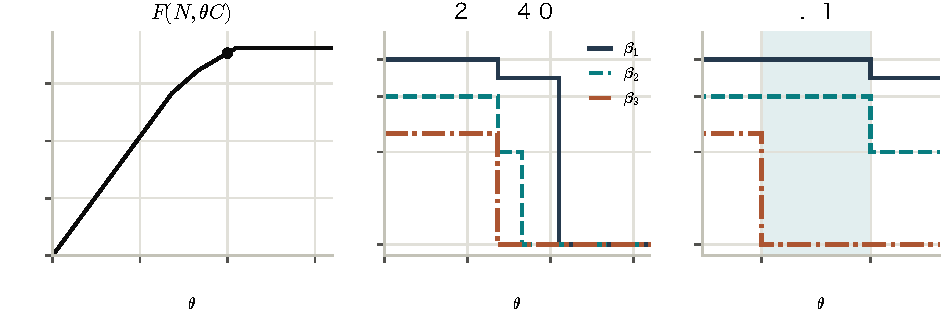
\includegraphics[width=\linewidth]{figures/lp_parametric.pdf}
\caption{库存缩放系数 $\theta$ 下的离线最优值 $F(N,\theta C)$（左）与库存影子价格 $\beta_j(\theta)$（右），$N=(50,30,20)$。竖线为课程实例 $\theta=1$}
\label{fig:parametric}
\end{figure}
